% This file contains both landscape and portrait mode slides.
% Choose one of the following to print them out:
%  - If using PSTricks, try the semcolor style option.
%  - If using Rokicki's dvips, try the semrot style option.
%  - To print {\em }the landscape slides, put \landscapeonly in the preamble.
%    To print the portrait slides, include the portrait style option and
%    put \portraitonly in the preamble.
%
%
\documentstyle[%
  fontenc,%
  colordvi,%
  graphicx,%
  epsfig,%
  rotating,%
  wrapfig,%
  epsf,%
  amsmath,%
  amsthm,%
  amsfonts,%
  picins,%
  fancybox,%
  %slidesonly,%  Try notes or notesonly instead.
  notes,%      Use instead of slidesonly to typeset the notes.
  %notesonly,%  Use instead of slidesonly to typeset notes and slides.
  semcolor,%   Try me if using PSTricks.
  semrot,%     Try me if using Rokicki's dvips.
  semhelv,%    Try me if using a PostScript printer.
  %article,%    Try me.
  portrait,%   Try me.
  %sem-a4,%     Try me if using A4 paper.
  semlayer%     This must be included, but you need the semcolor option to
  ]{seminar}                                  % actually see the overlays.

\slidesmag{4}
%\articlemag{1}

%\twoup                     % Try me for twoup printing.

%\portraitonly              % To print only portrait slides
%\landscapeonly             % To print only landscape slides

%\notslides{\ref{questions}-7,1}   %Try me: The slides are omitted.
%\onlyslides{\ref{questions}-7,1}  %Try me: Only these slides are included.
\onlynotestoo                     %Try me: For selecting notes as well.

\colorlayers{red,blue}      % Try deleting this if using the semcolor option,
                            % to get \blue and \red to use PostScript color.

%\overlaysfalse             % Suppress overlays with semcolor option.
%\layersfalse               % Suppress color layers with semcolor option.

\rotateheaderstrue          % Try this out if using rotation macros.

%%%%%%%%%%%%%%%%%%%%%%%%%%%%%%%%%%%%%%%%%%%%%%%%%%%%%%%%%%%%%%%%%%%%
%%% definitions des fontes
%
\newfont{\goth}{ygoth}
\newfont{\fancyet}{cmbxti10 scaled 700}
\newfont{\transf}{cmbx10}
%
%
%%%%%%%%%%%%%%%%%%%% dimensions %%%%%%%%%%%%%%%%%%%%%%
%
%\setlength{\textwidth}{18cm}
%\setlength{\textheight}{25cm}
%\setlength{\leftmargin}{-1cm}
%\setlength{\rightmargin}{1cm}
%\setlength{\topmargin}{-2.5cm}
%\setlength{\marginparwidth}{0cm}
%\setlength{\marginparsep}{-2.5cm}
%\setlength{\slideframesep}{8pt}
\setlength{\slidewidth}{8.75in}
\setlength{\slideheight}{7.2in}
\setlength{\slideframewidth}{1.5pt}
\renewcommand{\slideleftmargin}{0.2in}
\renewcommand{\sliderightmargin}{0.15in}
\renewcommand{\slidetopmargin}{1.0in}
\renewcommand{\slidebottommargin}{0.2in}
\renewcommand{\shadowthickness}{1pt}
\renewcommand{\slidefonts}{\transf}
%
%%%%%%%%%%%%%%%%%%%%%%%%%%%%%%%%%%%%%%%%%%%%%%%%%%%%%%%%%%%%%%%%%%%%
%%% redefinit les headers
%\newcommand{\sref}[1]{SLIDE \ref{#1}}
%\newcommand{\heading}[1]{\begin{center}\large\bf #1\end{center}}

\newpagestyle{MF}%
%  {{\tiny{Riad Suleiman}}\hfil\thepage}{}
  {{\tiny{ }}\hfil{\ }}{}
\pagestyle{MF}
%
%%%%%%%%%%%%%%%%%%%%%%%%%%%%%%%%%%%%%%%%%%%%%%%%%%%%%%%%%%%%%%%%%%%%
%%% include following to print two per page
%
%\twoup
%
%%%%%%%%%%%%%%%%%%%%%%%%%%%%%%%%%%%%%%%%%%%%%%%%%%%%%%%%%%%%%%%%%%%%
% Selective Section Processing
%
% note if you do not set option 'slidesonly', you will still get notes
% outside of the range specified here.
%
%\onlyslides{22-100}
%\includeonly{phys}
%\includeonly{curr_surv}
%\includeonly{delta}
%
%
%
%%%%%%%%%%%%%%%%%%%%%%%%%%%%%%%%%%%%%%%%%%%%%%%%%%%%%%%%%%%%%%%%%%%%
%%%%%%%%%%%%%%%%%%%%%%%%%%%%%%%%%%%%%%%%%%%%%%%%%%%%%%%%%%%%%%%%%%%%
%%
%gives greater than or approximately equal to
\def\gtorder{\mathrel{\raise.3ex\hbox{$>$}\mkern-14mu
             \lower0.6ex\hbox{$\sim$}}}
%give less than or approximately equal to
\def\ltorder{\mathrel{\raise.3ex\hbox{$<$}\mkern-14mu
             \lower0.6ex\hbox{$\sim$}}}
%%
%%%%%%%%%%%%%%%%%%%%%%%%%%%%%%%%%%%%%%%%%%%%%%%%%%%%%%%%%%%%%%%%%%%%
\begin{document}
\renewcommand{\slidefonts}{\transf}
%
%
%
% Title Slide and Outline
%%%%%%%%%%%%%%%%%%%%%%%%%%%%%%%%%%%%%%%%%%%%%%%%%%%%%%%%%%%%%%%%%%%%
\begin{slide*}

\begin{center}
\begin{shadowenv}[.45\slideheight]
\transf

\Blue{MySQL Interface for Parity } \\ 
{\ } \\
\end{shadowenv}
\end{center}

\vspace*{0.5cm}

\begin{center}
\normalsize
\transf{R.~Suleiman} \\
\vspace*{1.0cm}
%%\transf{\Magenta{$\mathcal{M}$assachusetts $\mathcal{I}$nstitute of 
%%$\mathcal{T}$echnology}} \\

\vspace*{1.0cm}
%%\transf{\scriptsize{(A Hall A Collaboration Proposal) \\
%%(New Proposal to Jefferson Lab PAC 19) }}\\
\end{center}

\vspace*{.3cm}
\begin{center}
\begin{shadowenv}[.3\slideheight]
\Red{\transf{Hall A Data Analysis Workshop}} \\
{\scriptsize{December 2001}}
\end{shadowenv}
\end{center}

\end{slide*}
%%%%%%%%%%%%%%%%%%%%%%%%%%%%%%%%%%%%%%%%%%%%%%%%%%%%%%%%%%%%%%%%

\begin{slide*}

\centerline{\shadowbox{\Blue{\Large Introduction}}}
{\Large 

\begin{itemize}
\item  The database is implemented in MySQL

{\Blue{\underline{\rm http://www.mysql.org}}}

\item C++ class (TaMysql) written in ROOT to 
interface with the database

{\Blue{\underline{\rm http://root.cern.ch}}}

\item Script to generate ascii files from the database, and one
to do the reverse, generate a database from the file: 

\begin{verbatim}
 > ascii2db.pl 

 > db2ascii.pl run=100
\end{verbatim}

\end{itemize}
}

\end{slide*}
%%%%%%%%%%%%%%%%%%%%%%%%%%%%%%%%%%%%%%%%%%%%%%%%%%%%%%%%%%%%%%%%

\begin{slide*}

\centerline{\shadowbox{\Blue{\Large Features}}}
{\Large 
\begin{itemize}
\item  For the "Pan" code, the database contains:

\begin{itemize}
     \item[1.] Logical Parameters that affect program flow
     \item[2.] DataMap (correspondence of 'keys' to event buffer)
     \item[3.] Calibration Parameters used by program
     \item[4.] Cuts and the event intervals associated
\end{itemize}

\item Run indexed lookup of constants

\item Keep a change log: user, date, time, comment

\end{itemize}
}

\end{slide*}
%%%%%%%%%%%%%%%%%%%%%%%%%%%%%%%%%%%%%%%%%%%%%%%%%%%%%%%%%%%%%%%%

\begin{slide*}

\centerline{\shadowbox{\Blue{\Large Ascii Database}}}

\tiny

\begin{verbatim}

# Default control file.  If the file for your run is not
# around, this file will be used to control the code.
    runtype BEAM      
    lobeam  12000   # cut to define beam too low 
    burpcut 5000    
    oversamp  10    # oversampling factor
    windelay  8     # helicity delay in windows
    pairtype  quad  
    dacnoise adc 0 chan 0 slope 0.901 int 42.1  
    dacnoise adc 0 chan 1 slope 0.902 int 42.2  
    dacnoise adc 1 chan 0 slope 0.911 int 44.1  
    dacnoise adc 1 chan 1 slope 0.912 int 44.2  
    dacnoise adc 2 chan 0 slope 0.921 int 44.1  
    dacnoise adc 2 chan 1 slope 0.922 int 44.2  
    ped adc 0 chan 0 value 101.3
    ped adc 0 chan 1 value 103.3
    ped adc 1 chan 0 value 111.3
    ped adc 1 chan 1 value 113.3
    ped adc 2 chan 0 value 121.3
    ped adc 2 chan 1 value 123.3
    header adc       ffadc000 fffff000    
    header timeboard fffbd000 fffff000   
    header tir       ffdaf000 fffff000    
    header scaler    fffca000 fffff000  
#   table  device-type device-name adc startchan evbuff-offset channel-names(keys)
    datamap   bcm        bcm1       0    0         22             bcm1
    datamap   bcm        bcm2       0    3         24             bcm2
    datamap   bpm        bpm8       1    0         30    bpm8xp bpm8xm bpm8yp bpm8ym
    datamap   tir        tir        0    0         34        helicity realtime 
    datamap   timeboard  timeboard  0    0          0               dac
    ncuts 14        
    evlo 10 10 10 10 10 10 0 0 0 0 20 20 40 30
    evhi 40 40 40 40 40 20 0 0 0 0 60 60 70 60
    evint 21232  23442 4  1
    evint 32232  34554 6  1
    evint 35665  37440 4  1
    evint 42112  43443 7  1
    evint 56712  58142 8  1

\end{verbatim}


\end{slide*}
%%%%%%%%%%%%%%%%%%%%%%%%%%%%%%%%%%%%%%%%%%%%%%%%%%%%%%%%%%%%%%%%

\begin{slide*}

\centerline{\shadowbox{\Blue{\Large Database Schematic }}}

\begin{figure}[htbp]
\begin{center}
%\htmlimage{thumbnail=1.0}
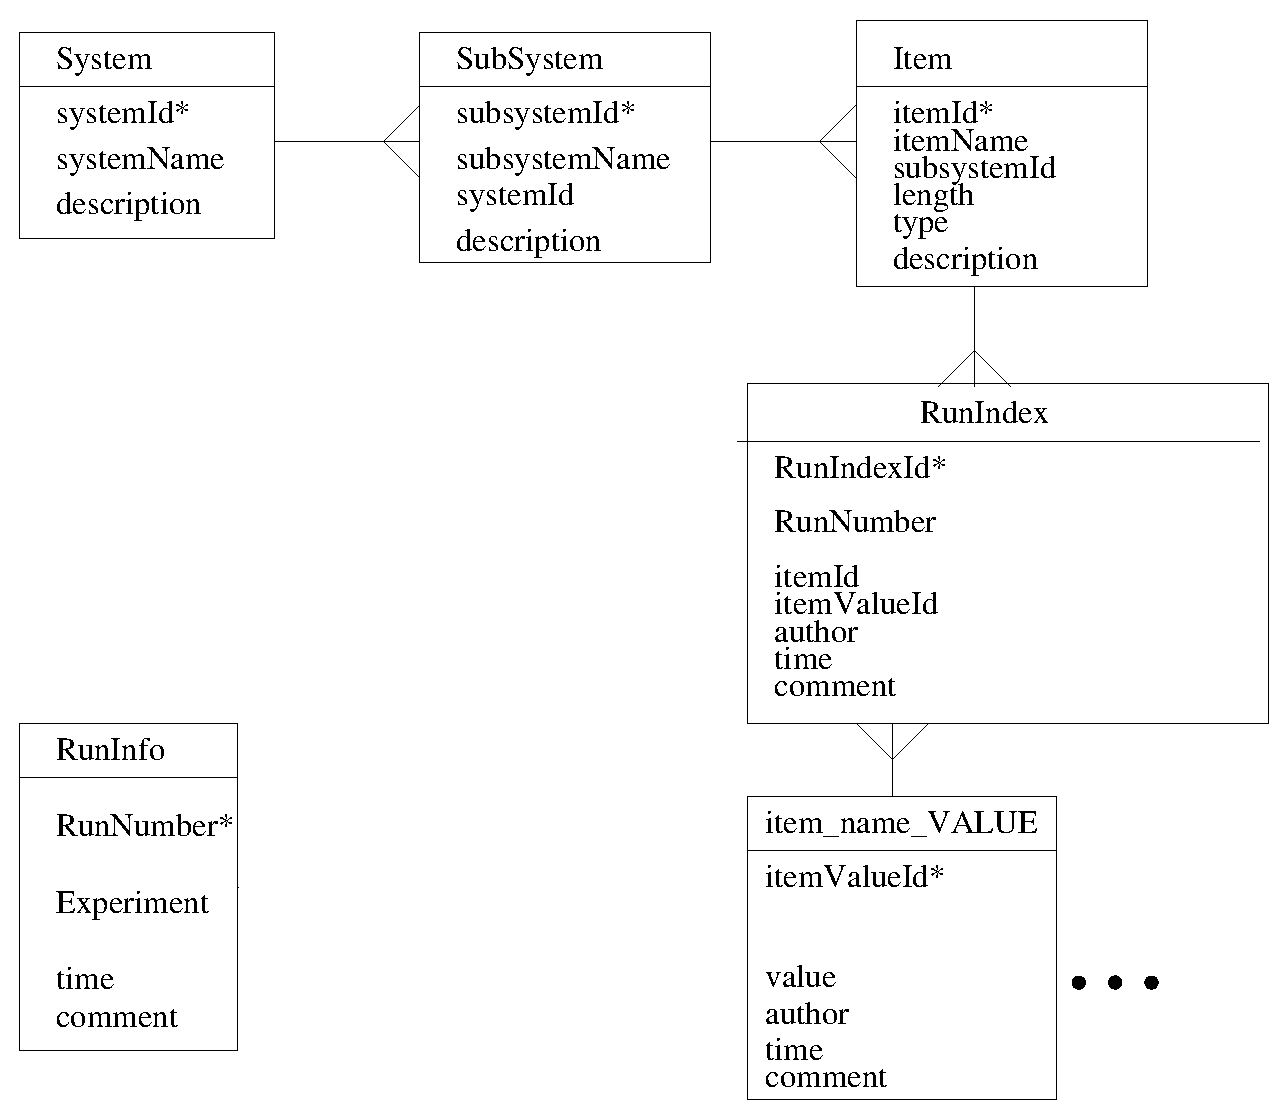
\epsfig{file=dbdiag.eps, height=.4\slidewidth, width=0.4\slideheight}
\end{center}
\end{figure} 

\end{slide*}
%%%%%%%%%%%%%%%%%%%%%%%%%%%%%%%%%%%%%%%%%%%%%%%%%%%%%%%%%%%%%%%%

\begin{slide*}

\centerline{\shadowbox{\Blue{\Large Database Tables }}}

\tiny

\begin{table}[htbp]
\begin{center}
\begin{tabular}{|l|l|l|l|} \hline
\multicolumn{4}{|c|}{RunInfo} \\ \hline
column name & type & example & comment \\ \hline\hline
RunNumber   & int        & 2000        & Primary key \\
Experiment  &  varchar   &  ``HAPPEXII'' &  \\
time        & datetime   &  2003-12-09 11:30:45&  \\
comment     & text       &             &  \\ \hline
\end{tabular}
\end{center}
\end{table}


\begin{table}[htbp]
\begin{center}
\begin{tabular}{|l|l|l|l|} \hline
\multicolumn{4}{|c|}{System} \\ \hline
column name & type & example & comment \\ \hline\hline
systemId    & int     & 1              & Primary key auto increment\\
systemName  & varchar & ``dacnoise'' &  \\
description & text    &                & \\ \hline
\end{tabular}
\end{center}
\end{table}


\begin{table}[htbp]
\begin{center}
\begin{tabular}{|l|l|l|l|} \hline
\multicolumn{4}{|c|}{SubSystem} \\ \hline
column name & type & example & comment \\ \hline\hline
subsystemId    & int     &  1           & Primary key auto increment\\
subsystemName  & varchar & ``adc0'' & \\
systemId       & int     &  1           & Foreign key reference System\\
description    & text    &              & \\ \hline
\end{tabular}
\end{center}
\end{table}


\begin{table}[htbp]
\begin{center}
\begin{tabular}{|l|l|l|l|} \hline
\multicolumn{4}{|c|}{Item} \\ \hline
column name & type & example & comment \\ \hline\hline
itemId      & int     & 1         & Primary key auto increment\\
itemName    & varchar & ``chan0''   & \\
subsystemId & int     & 1         & Foreign key reference SubSystem\\
length      & int     & 2         & Number of elements\\
type        & varchar & ``float'' & \\
description & text    &           & \\ \hline
\end{tabular}
\end{center}
\end{table}


\begin{table}[htbp]
\begin{center}
\begin{tabular}{|l|l|l|l|} \hline
\multicolumn{4}{|c|}{RunIndex} \\ \hline
column name & type & example & comment\\ \hline\hline
RunIndexId     & int        & 1       & Primary key auto increment\\
RunNumber      & int        & 2000   &  \\
itemId         & int        & 1       & Foreign key reference Item\\
itemValueId    & int        & 1       & Foreign key reference item\_name\_VALUE\\
author         & varchar     & ``dbmanager''            & \\
time           & timestamp  & 20000502165717        & \\ 
comment        & text       &                       & \\ \hline
\end{tabular}
\end{center}
\end{table}


\begin{table}[htbp]
\begin{center}
\begin{tabular}{|l|l|l|l|} \hline
\multicolumn{4}{|c|}{dacnoise\_adc0\_chan0\_VALUE} \\ \hline
column name & type & example & comment\\ \hline\hline
itemValueId    & int        &  1       & Primary key auto increment\\
value\_1       & ``float''   &  1.82    &  \\
author         & varchar    & ``smith''& \\
time           & timestamp  & 20000502165717 & \\ 
comment        & text       &                & \\ \hline
\end{tabular}
\end{center}
\end{table}


\centerline{$\vdots$}


\begin{table}[htbp]
\begin{center}
\begin{tabular}{|l|l|l|l|} \hline
\multicolumn{4}{|c|}{\hspace*{0.8in} $\ldots$ \_VALUE \hspace*{0.8in}} \\ \hline
\end{tabular}
\end{center}
\end{table}

\centerline{$\vdots$}

\end{slide*}
%%%%%%%%%%%%%%%%%%%%%%%%%%%%%%%%%%%%%%%%%%%%%%%%%%%%%%%%%%%%%%%%

\begin{slide*}

\centerline{\shadowbox{\Blue{\Large Access Privilege}}}

{\Large

There are two different levels of access to the database:

\begin{itemize}
\item{} database manager
\item{} users
\end{itemize}
}

\begin{table}[htbp]
\begin{center}
\begin{tabular}{|l|l|l|l|} \hline
\multicolumn{4}{|c|}{user table}\\ \hline
      Host                & User      & Password & Privileges \\ \hline\hline
      localhost           & dbmanager & non-NULL & none \\
      \%                  & dbuser      & NULL     & none \\ \hline
\end{tabular}
\caption{MySQL user table. Any user from any host can connect to the database.}
\label{usertable}
\end{center}
\end{table}

\begin{table}[htbp]
\begin{center}
\begin{tabular}{|l|l|l|l|} \hline
\multicolumn{4}{|c|}{db table}\\ \hline
      Host  & Db     &User      &Privileges\\ \hline\hline
       \%   &  pandb & dbmanager& all\\
       \%   &  pandb & \%       &  select\\ \hline
\end{tabular}
\caption{MySQL db table. The dbmanager has all privileges in the pandb
database. Any user that can connect can read any of the tables in the
pandb database.}
\label{dbtable}
\end{center}
\end{table}


\end{slide*}
%%%%%%%%%%%%%%%%%%%%%%%%%%%%%%%%%%%%%%%%%%%%%%%%%%%%%%%%%%%%%%%%

\begin{slide*}

\centerline{\shadowbox{\Blue{\Large Web Interface}}}

\vspace*{1in}

{\Large
\begin{itemize}

\item[-] dbuser:

{\Blue{\underline{\rm http://alquds.jlab.org/panDB}}}

\vspace*{0.5in}


\item[-] dbmanager:

{\Blue{\underline{\rm http://alquds.jlab.org/pandb}}}

\end{itemize}
}

\end{slide*}
%%%%%%%%%%%%%%%%%%%%%%%%%%%%%%%%%%%%%%%%%%%%%%%%%%%%%%%%%%%%%%%%


\end{document}
